\section{Design mécanique}\label{sec:mecanique}

Le design mécanique de la station a été entièrement revu par rapport aux
concepts initiaux. L'objectif était de concevoir un boîtier à la fois
compact, résistant aux intempéries et offrant une ventilation passive
suffisante pour que les mesures de température et d'humidité ne soient
pas biaisées par l'échauffement interne.

\subsection{Structure intérieure}\label{subsec:interieur}

Les deux PCB sont empilés verticalement sur des entretoises filetées,
formant une structure en deux étages analogue à un rack miniaturisé.
Cette architecture présente plusieurs avantages :

\begin{itemize}
  \item Chaque étage est démontable indépendamment, ce qui facilite la
    maintenance et le débogage.
  \item La forme circulaire des PCB optimise l'occupation du volume
    cylindrique disponible à l'intérieur du boîtier.
  \item Les connecteurs inter-étages sont positionnés pour minimiser la
    longueur des câbles.
\end{itemize}

Des prototypes de la structure intérieure ont été réalisés par découpe
laser sur MDF, permettant de valider les cotes, les positions de fixation
et l'accessibilité aux connecteurs avant la commande des PCB définitifs
(figure~\ref{fig:interieur}).

\begin{figure}[H]
  \centering
  \begin{subfigure}[b]{0.48\textwidth}
    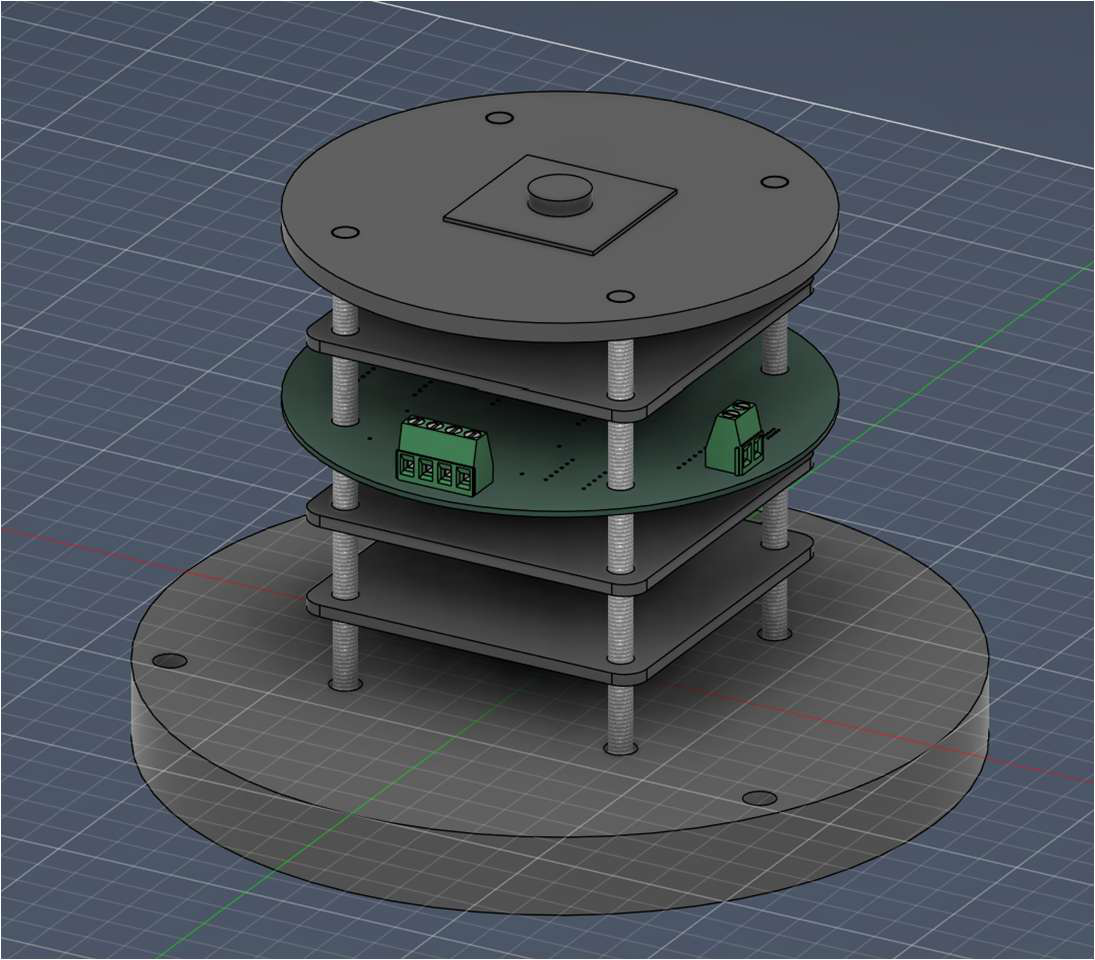
\includegraphics[width=\textwidth]{images/mecanique_interieur_cao.png}
    \caption{Rendu CAO}
  \end{subfigure}
  \hfill
  \begin{subfigure}[b]{0.48\textwidth}
    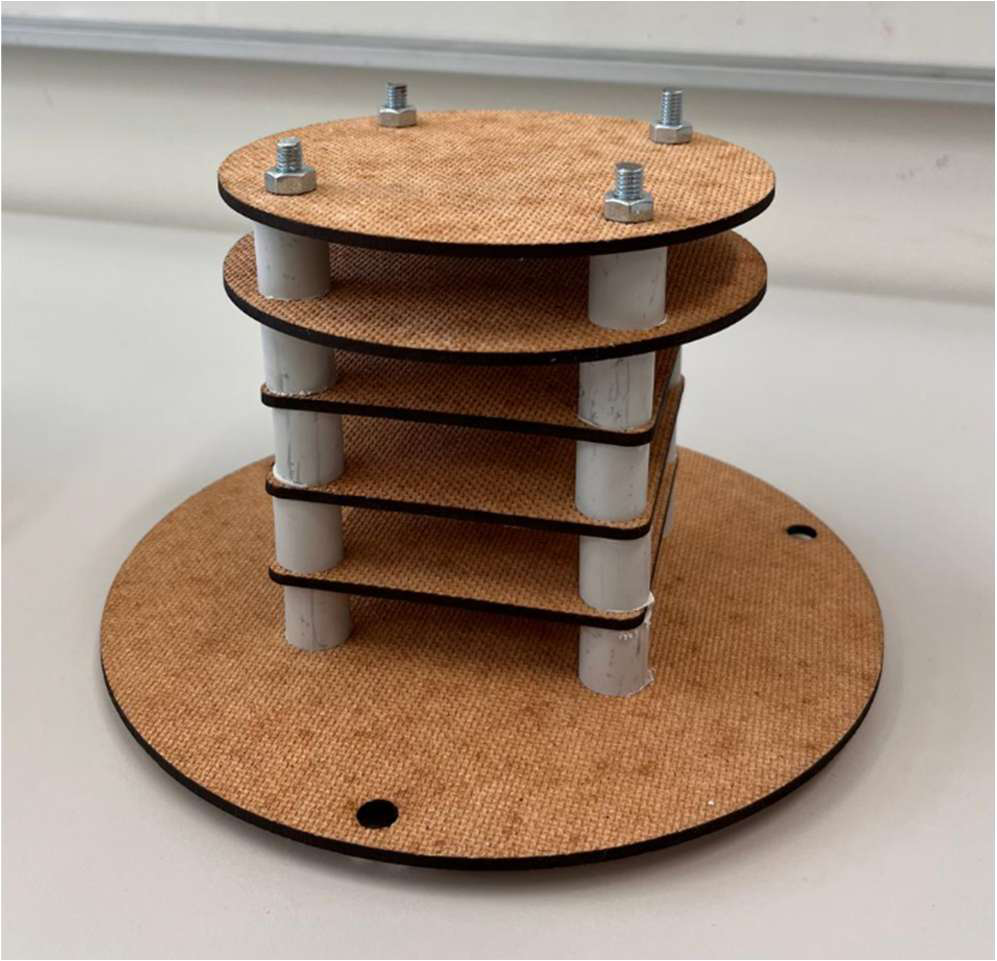
\includegraphics[width=\textwidth]{images/mecanique_interieur_photo.png}
    \caption{Prototype MDF}
  \end{subfigure}
  \caption{Structure intérieure : empilement des PCB sur entretoises.}
  \label{fig:interieur}
\end{figure}

\subsection{Boîtier extérieur}\label{subsec:exterieur}

Le boîtier extérieur s'inspire du principe de l'\textit{abri de Stevenson},
un standard météorologique historique conçu pour protéger les instruments
de mesure du rayonnement solaire direct et des précipitations, tout en
permettant la libre circulation de l'air. Notre version adapte ce concept
à une géométrie cylindrique compacte, plus adaptée à une fixation sur un
mât ou une rambarde de voilier.

La station se compose de deux parties distinctes :

\begin{itemize}
  \item \textbf{Partie basse (blanche)} : corps cylindrique en plastique blanc
    à faible absorption solaire. Des ouvertures latérales permettent la
    circulation de l'air autour des capteurs atmosphériques tout en
    bloquant les projections directes d'eau.
  \item \textbf{Chapeau supérieur (noir)} : capot orienté vers le ciel
    qui accueille la caméra sous un dôme en plexiglas transparent pour
    l'acquisition d'images nuageuses.
\end{itemize}

Des prototypes de cette enveloppe ont été réalisés en impression 3D
(PLA et PETG), permettant de valider l'assemblage et l'étanchéité des
jointures avant d'envisager des matériaux plus durables pour une
utilisation marine prolongée. Des membranes \textit{Gore-Tex} ont
également été intégrées dans les tests pour évaluer leur capacité à
assurer la ventilation tout en empêchant les entrées d'eau.

\begin{figure}[H]
  \centering
  \begin{subfigure}[b]{0.48\textwidth}
    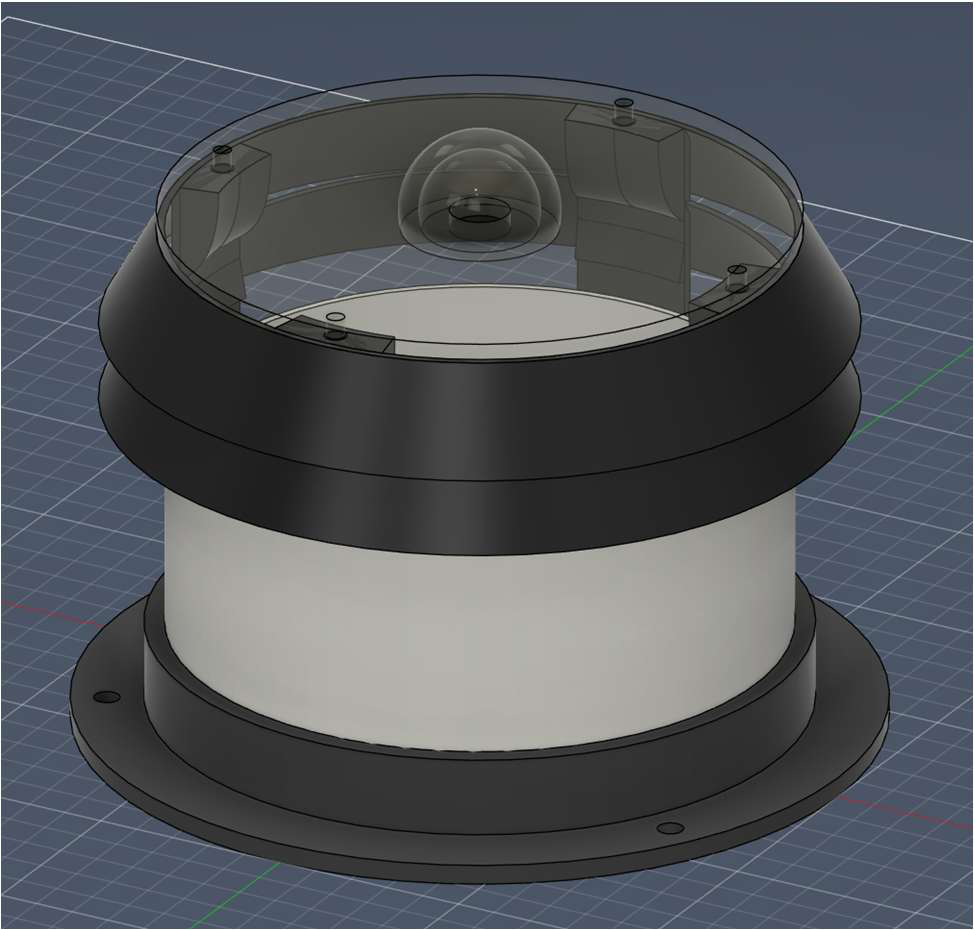
\includegraphics[width=\textwidth]{images/mecanique_boitier_cao.png}
    \caption{Rendu CAO}
  \end{subfigure}
  \hfill
  \begin{subfigure}[b]{0.48\textwidth}
    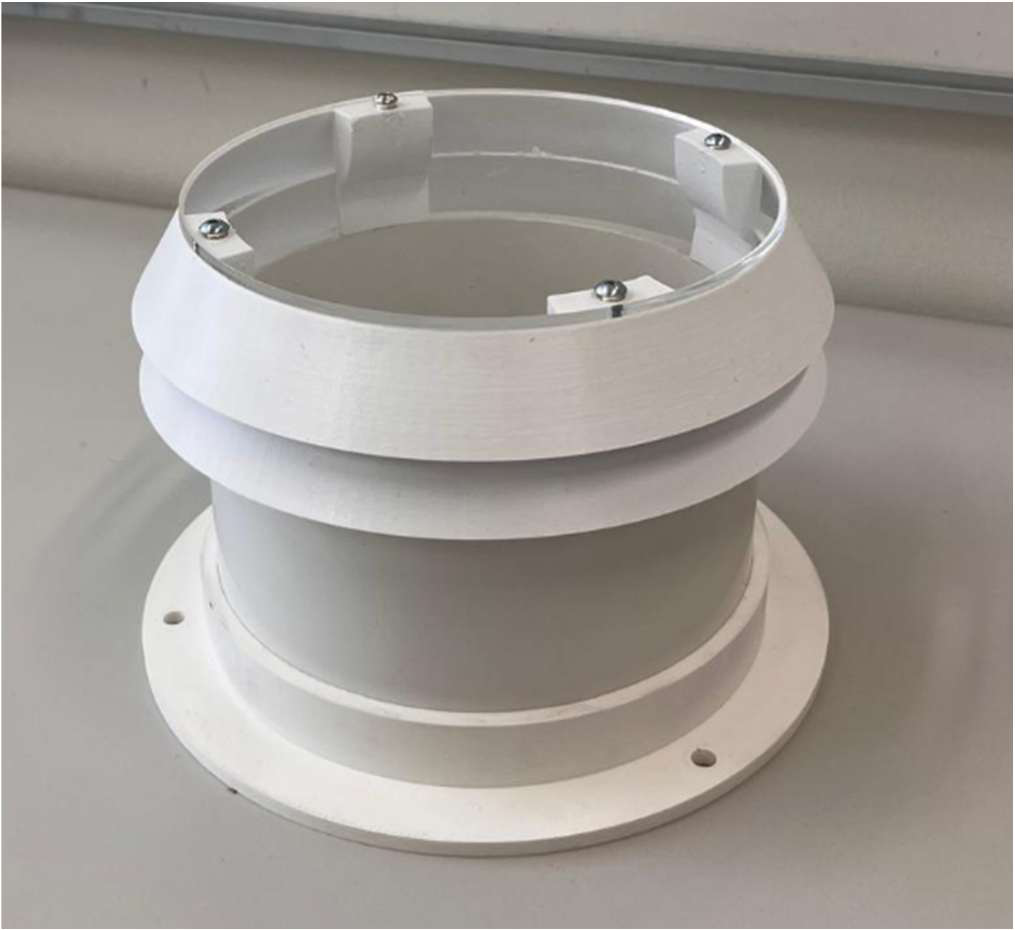
\includegraphics[width=\textwidth]{images/mecanique_boitier_photo.png}
    \caption{Prototype imprimé 3D}
  \end{subfigure}
  \caption{Boîtier extérieur : chapeau noir (caméra) et corps blanc (ventilation).}
  \label{fig:exterieur}
\end{figure}

\begin{figure}[H]
  \centering
  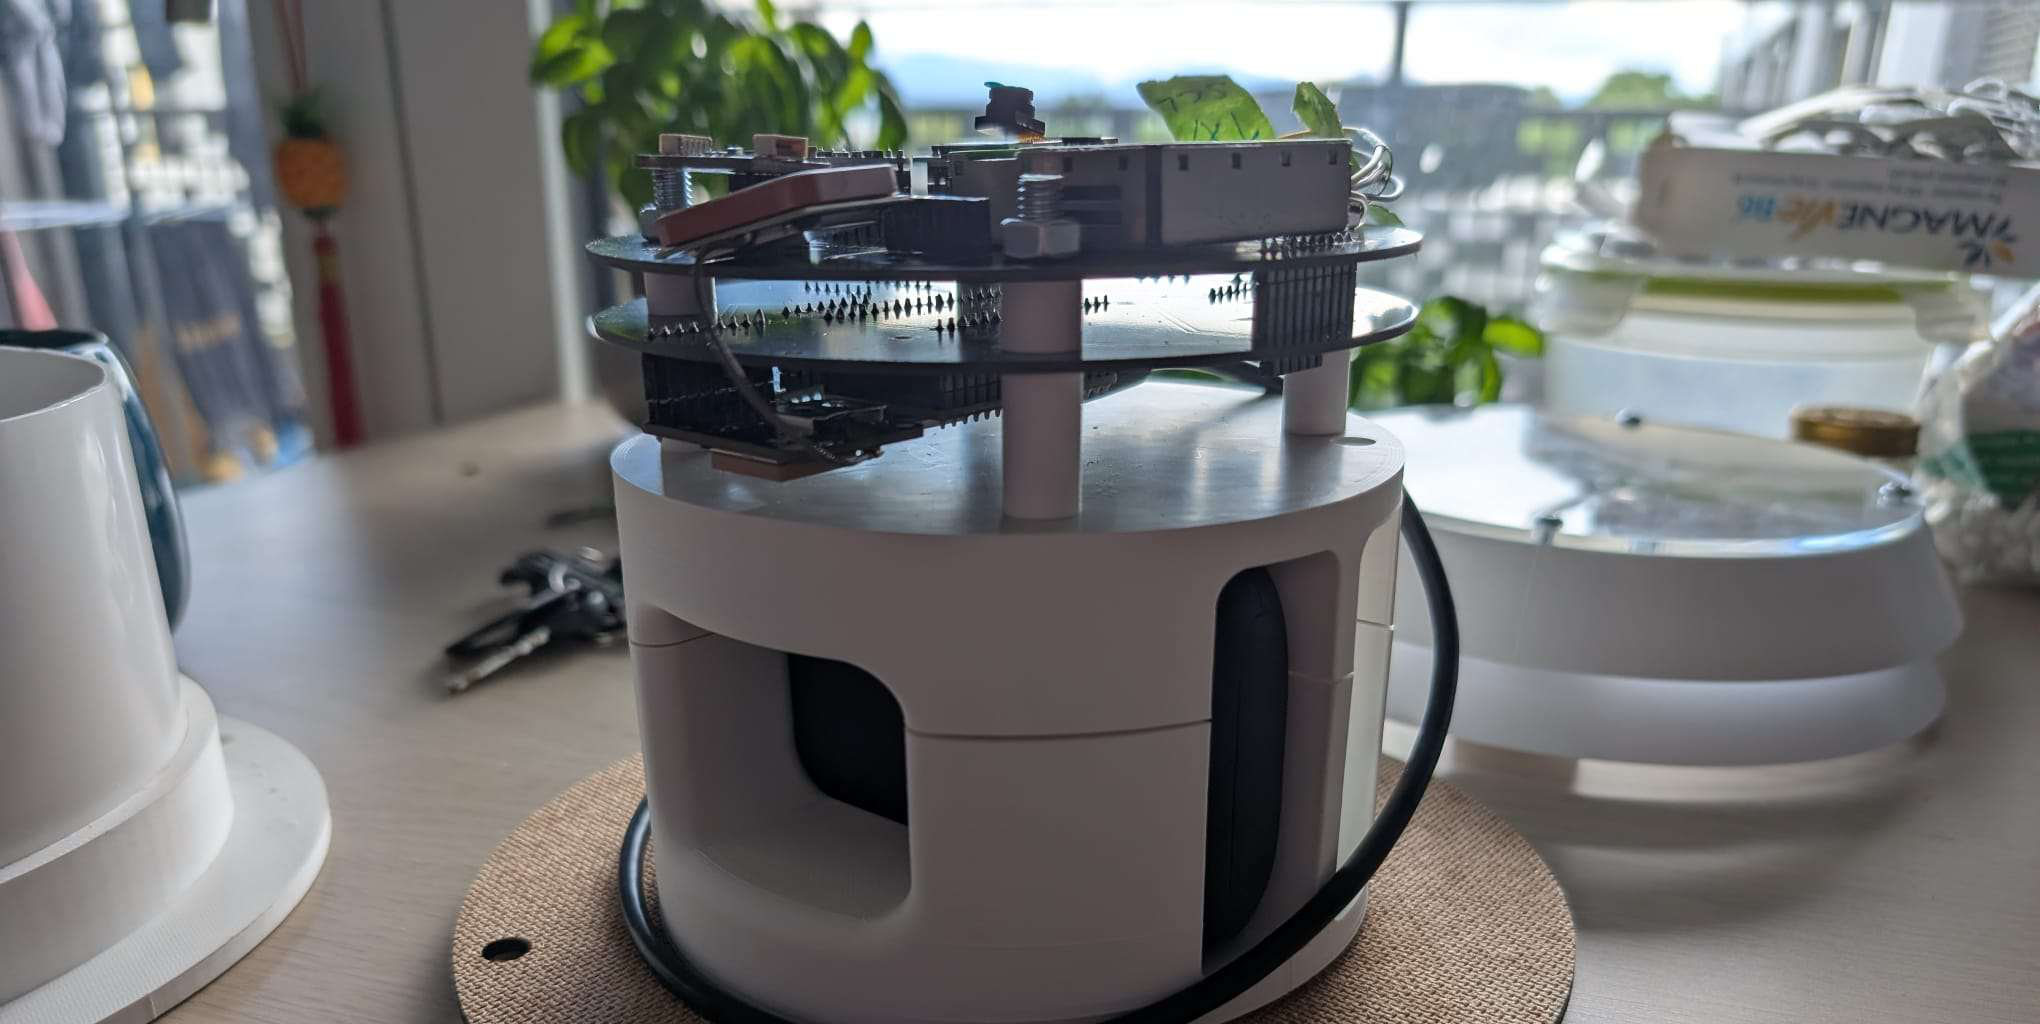
\includegraphics[width=0.5\textwidth]{images/station_assemblée.png}
  \caption{Station assemblée avec les PCBs montés sur la structure intérieure.}
  \label{fig:station_assemblée}
\end{figure}

\subsection{Problèmes identifiés et solutions}\label{subsec:problemes_meca}

Deux risques ont été identifiés lors des tests préliminaires et font
l'objet d'investigations spécifiques.

\paragraph{Effet de serre lié au dôme en plexiglas.}
Le plexiglas est transparent au rayonnement visible mais partiellement
opaque au rayonnement infrarouge thermique. Il pourrait donc créer un
effet de serre local sous le capot supérieur, biaisant les mesures de
température et d'humidité si les capteurs se trouvent à proximité. Des
mesures comparatives sont prévues pour quantifier cet écart. Si l'effet
est significatif, la plaque supérieure sera remplacée par un matériau
ajouré ou traité antireflet, ou les capteurs sensibles seront déplacés
vers la partie basse du boîtier.

\paragraph{Ventilation suffisante.}
L'abri de Stevenson repose sur la convection naturelle. Sur un voilier
en mouvement, le vent relatif est généralement suffisant pour assurer
un renouvellement d'air permanent. Pour les situations de calme plat,
une alternative basée sur un tube en coude (aspiration passive par
effet venturi du vent résiduel) a été envisagée. Cette solution
nécessiterait toutefois l'ajout d'un ventilateur en l'absence de vent,
ce qui augmente la complexité et la consommation électrique. Les tests
en conditions réelles permettront de trancher.

\begin{figure}[H]
  \centering
  \begin{subfigure}[b]{0.35\textwidth}
    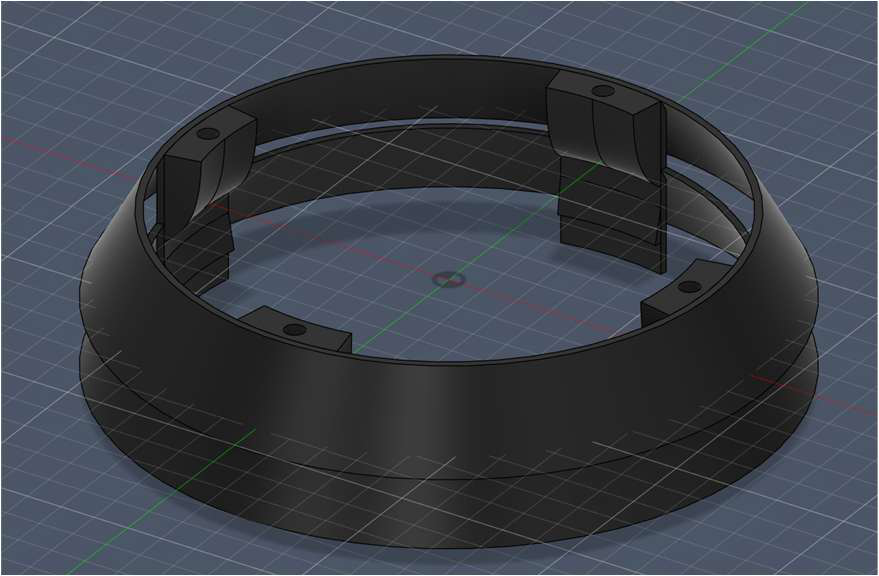
\includegraphics[width=\textwidth]{images/mecanique_stevenson_anneau.png}
    \caption{Anneau de ventilation (CAO)}
  \end{subfigure}
  \hfill
  \begin{subfigure}[b]{0.55\textwidth}
    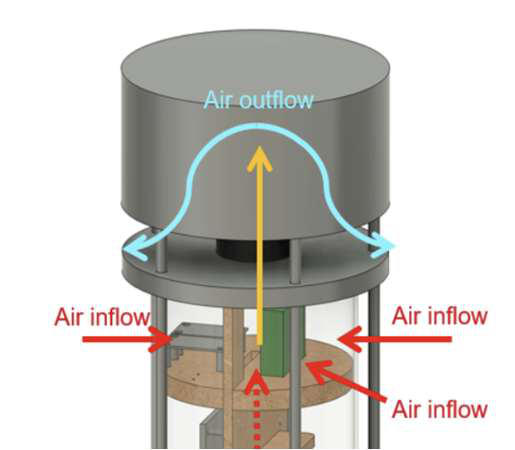
\includegraphics[width=\textwidth]{images/mecanique_ventilation.png}
    \caption{Schéma de circulation d'air}
  \end{subfigure}
  \caption{Ventilation passive : entrées d'air latérales et sortie par le haut.}
  \label{fig:ventilation}
\end{figure}
